%% The first command in your LaTeX source must be the \documentclass command.
%%
%% Options:
%% twocolumn : Two column layout.
%% hf: enable header and footer.
\documentclass[
% twocolumn,
% hf,
]{ceurart}

%%
%% One can fix some overfulls
\sloppy

%%
%% Minted listings support 
%% Need pygment <http://pygments.org/> <http://pypi.python.org/pypi/Pygments>
\usepackage{listings}
\usepackage{amsmath}
\usepackage{multirow}
\usepackage{graphicx}
\usepackage{caption}
\usepackage{subcaption}
\usepackage{threeparttable}
\graphicspath{ {./img/} }
%% auto break lines
\lstset{breaklines=true}

% \newcommand{\newrev}[1]{{\textbf{{\color{blue}#1}}}}
\newcommand{\newrev}[1]{{{#1}}}

\newcommand{\CellWithForceBreak}[2][c]{
\begin{tabular}[#1]{@{}c@{}}#2\end{tabular}}

%%
%% end of the preamble, start of the body of the document source.
\begin{document}

%%
%% Rights management information.
%% CC-BY is default license.
\copyrightyear{2022}
\copyrightclause{Copyright for this paper by its authors.
  Use permitted under Creative Commons License Attribution 4.0
  International (CC BY 4.0).}

%%
%% This command is for the conference information
\conference{To be decided}

%%
%% The "title" command
\title{An Analytical Framework for Knowledge Wealth of Knowledge Graphs}

% \tnotemark[1]
% \tnotetext[1]{You can use this document as the template for preparing your
%   publication. We recommend using the latest version of the ceurart style.}

%%
%% The "author" command and its associated commands are used to define
%% the authors and their affiliations.
\author[1]{TBD}[%
% orcid=0000-0002-0877-7063,
email=tbd@ui.ac.id,
% url=https://yamadharma.github.io/,
]
% \cormark[1]
% \fnmark[1]
\author[1]{TBD}[%
% orcid=0000-0002-0877-7063,
email=tbd@ui.ac.id,
% url=https://yamadharma.github.io/,
]
% \cormark[1]
% \fnmark[1]
\address[1]{Faculty of Computer Science, Universitas Indonesia, Depok, Indonesia}

\author[2]{TBD}[%
% orcid=0000-0001-7116-9338,
email=tbd@catapa.com,
% url=https://kmitd.github.io/ilaria/,
]
% \fnmark[1]
\address[2]{CATAPA, Jakarta, Indonesia}

\author[3]{TBD}[%
% orcid=0000-0002-9421-8566,
email=tbd@gdplabs.id,
% url=http://conceptbase.sourceforge.net/mjf/,
]
% \fnmark[1]
\address[3]{GDP Labs, Jakarta, Indonesia}

%% Footnotes
% \cortext[1]{Corresponding author.}
% \fntext[1]{These authors contributed equally.}

%%
%% The abstract is a short summary of the work to be presented in the
%% article.
\begin{abstract}
Along with the rapid development of data volumes, the need for machine-readable data is inevitable. As a result, the use of knowledge graph data structures becomes more popular. With its development, quality aspects of a knowledge graph need to be considered, one of which is knowledge wealth: the amount of information contained in a knowledge graph. A high level of knowledge wealth in a knowledge graph may indicate the high quality of a knowledge graph; conversely, a low level of knowledge wealth can be a sign of poor quality of a knowledge graph. However, there is no formal way to define knowledge wealth and how to measure and analyze it. This study proposes a framework to analyze knowledge wealth and the level of knowledge imbalance in the RDF knowledge graph by seeing how the knowledge wealth of an entity class is spread over the knowledge graph using statistical measures and visualization. In addition, this framework also helps to identify entity groups based on the level of wealth in their class, finds the best theoretical distribution that fits best to knowledge wealth distribution, performs clustering on classes based on the shape of knowledge wealth distribution, and detects bias in a knowledge graph. To evaluate this framework, some use cases were conducted on several classes on Wikidata. It is hoped that the results of this study can assist in researching knowledge wealth in the knowledge graph and be used to optimize the efforts of editing and developing knowledge graph projects by the contributors.
\end{abstract}

%%
%% Keywords. The author(s) should pick words that accurately describe
%% the work being presented. Separate the keywords with commas.
\begin{keywords}
  Knowledge graphs \sep
  knowledge wealth \sep
  knowledge imbalance analysis
\end{keywords}

%%
%% This command processes the author and affiliation and title
%% information and builds the first part of the formatted document.
\maketitle


%% include motivating scenario
\section{Introduction}

Our study proposes a formal model of knowledge wealth in the RDF knowledge graph by seeing how the knowledge wealth of an entity class is spread over the knowledge graph using statistical measures and visualization. In addition, a comprehensive analytical framework is also contructed that would give insights about the wealth of a class, the inequality between classes, and similarity of class distributions. To evaluate this framework, some use cases were conducted on \textbf{several <here change to exact number>} classes on Wikidata.

\section{Related Work}
\paragraph{Data Completeness Profiling} Wisesa et al. (2019) presented ProWD, a framework and web application tool for profiling the completeness of Wikidata. It is used to provide insight on degree of attribute completeness of a class in Wikidata. The visualization provided in the we dashboard is equipped with single, compare, or multidimensional view to help in analyzing the facet at entity or class level.

\paragraph{Imbalance and Gap in Wikidata}
- Refo: Gini index


- Nio: gap property
Ramadizsa1 et al. (2023) introduced the concept of gap properties that helps to characterize class-level knowledge gaps within knowledge graphs. The framework adapts association rule mining to determine ...


\section{Knowledge Wealth Analytics Framework}

\subsection{Wealth Formal Model}
Knowledge graphs follow Resource Description Framework (RDF) as a means of data organization. Data is stored in the form of triple \((S, p, o)\); a combination of a subject \(S\), a predicate \(p\), and an object \(o\) which can be visualized as nodes and directed-arc diagrams. For example, the statement "William Shakespeare's notable work is Romeo and Juliet" is mapped to the triple (\textit{WilliamShakespeare}, \textit{notableWork}, \textit{RomeoAndJuliet}).

There are 3 kind of nodes: IRIs, literals, and blank nodes. A triple is in the form of \((S, p, o) \in G) \cap (I \cup B) \times I \times (I \cup B \cup L) \) where \(I\) is the node with type IRIs, \(B\) is the node with type of blank node, and \(L\) is the node with type of literals.

\subsubsection{Class}
In this study, we re-use the class model defined by Ramadizsa1 et al. (2023). A class is a group of entities that are the subject of the study. \textit{Human}, \textit{film}, and \textit{taxon} are some examples of class. In general, entity \(S\) is an instance of class \(C\) is expressed by the triple (\(S\), \textit{instanceOf}, \(C\)). We can get a more narrow class inside the defined class by specifying additional conditions, each consisting of a particular property and value associated with it. Example of such conditions for human class is \textit{gender} with associated value \textit{male}, while example for a country would be \textit{continent} with value \textit{Asia}. For instance, the class of human with gender male that lived during English Renaissance is queried using
\[
    (?S, \{(?S, instanceOf, Human), (?S, gender, male), (?S, timePeriod, EnglishRenaissance)\})
\]

\subsubsection{Entity-Level Wealth: Knowledge Wealth Type and Definition}

\begin{figure}
     \centering
     \begin{subfigure}[b]{0.3\textwidth}
         \centering
         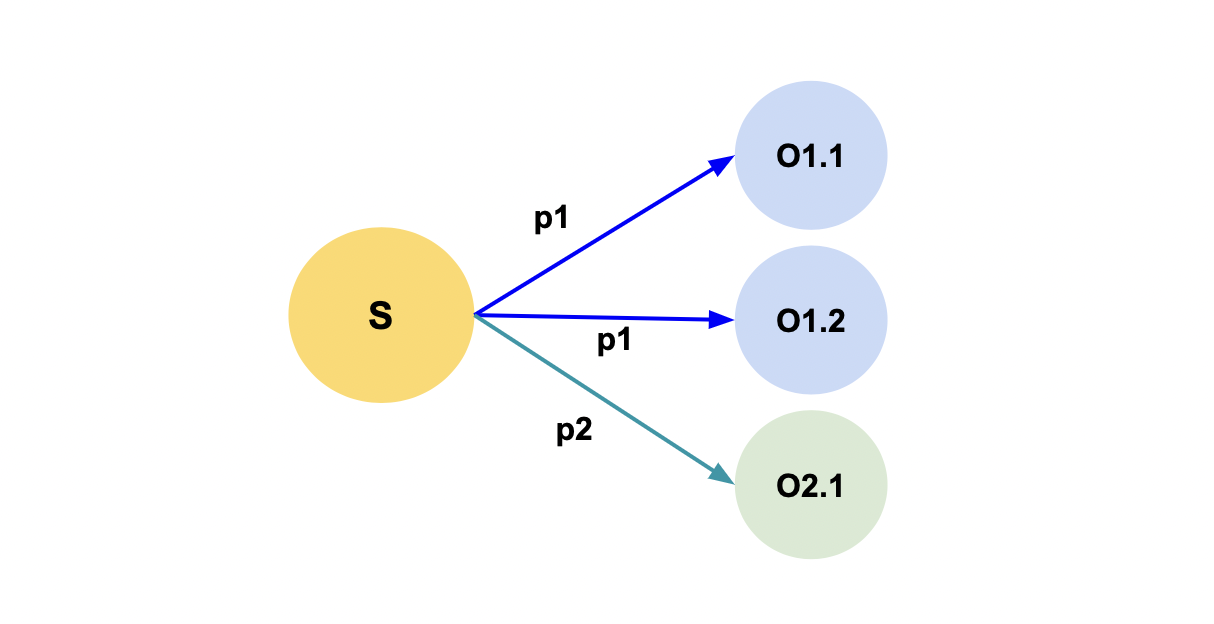
\includegraphics[scale=.3]{Wealth Type 1}
         \caption{Illustration of bag of properties and set of properties}
         \label{fig:wealth-type1}
     \end{subfigure}
     \hfill
     \begin{subfigure}[b]{0.3\textwidth}
         \centering
         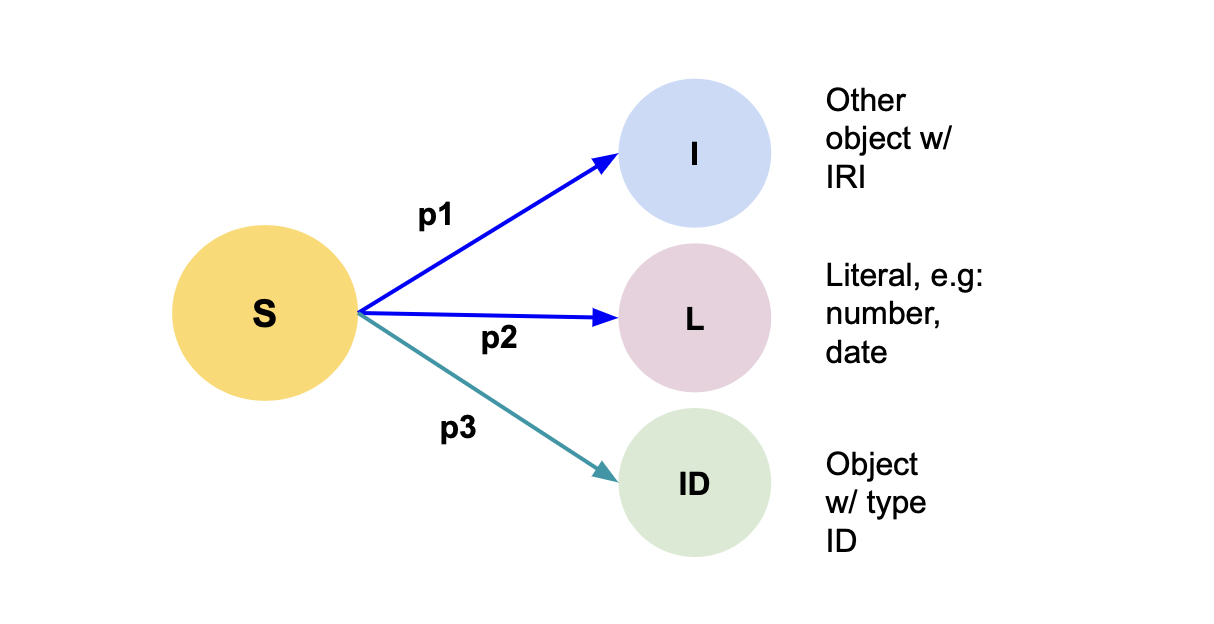
\includegraphics[scale=.3]{Wealth Type 2}
         \caption{Illustration of 3 types of property: object, literal, ID}
         \label{fig:wealth-type2}
     \end{subfigure}
     \hfill
     \begin{subfigure}[b]{0.3\textwidth}
         \centering
         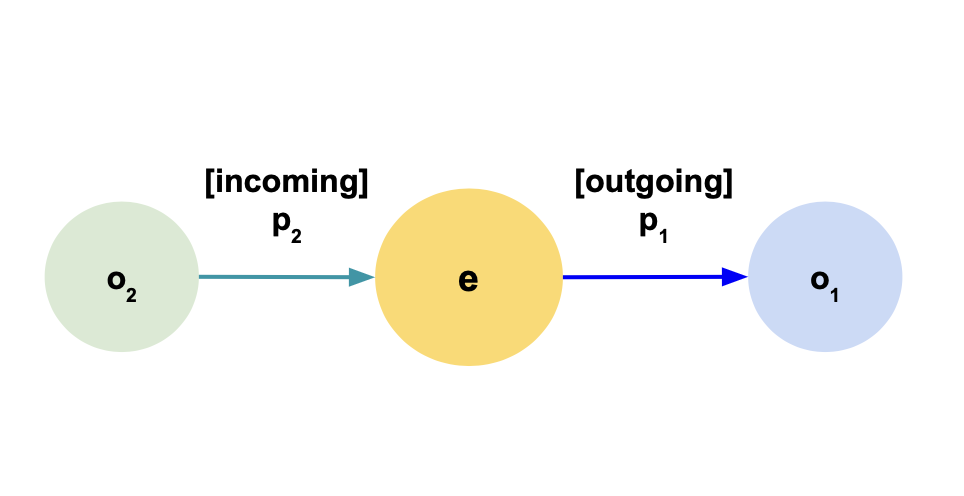
\includegraphics[scale=.3]{Wealth Type 3}
         \caption{Illustration of incoming link vs. outgoing link}
         \label{fig:wealth-type3}
     \end{subfigure}
     \caption{Three simple graphs}
     \label{fig:three graphs}
\end{figure}

Let \(S\) be any entity in a knowledge graph \(G\). We quantify the wealth of entity \(S\) in \(G\) as the amount of information about \(S\) available in \(G\). Thus, the knowledge wealth of an entity is defined by the number of properties associated/linked to it. For example, the wealth of William Shakespeare (Q692) in Wikidata counts all triples describing Q692 in Wikidata, including those detailing his family, occupation, image, and so on.

There are several notion on how to calculate the knowledge wealth of an entity: (1) wealth based on the (non-)uniqueness of individual property; (2) wealth based on type of property; and (3) wealth based on the direction of the link. The wealth of \(S\) with regard to graph \(G\) for each wealth category is denoted by \(W\), formalized and explained as follows.

\paragraph{Wealth based on the (non-)uniqueness of individual properties}
The first measure of the knowledge wealth of \(S\) is bag of properties---the cardinality of set of all triples that has \(S\) in their subject position. In this definition, the triples \((S, p_1, o_1)\) and \((S, p_1, o_2)\) account for a wealth of 1 each, thus both have a total of 2.
Let \(N_{bag}(S,G)\) be a set that comprises all pair of predicate/property and object \((p,o)\) that is connected to \(S\). Then \(W_{bag}(S, G)\) is the cardinality of \(N_{bag}(S,G)\).
\[
    N_{bag}(S,G) = \{(p, o) | (S, p, o) \in G\}
\]
\[
    W_{bag}(S,G) = |N_{bag}(S)|
\]

Another way of measuring the wealth is by counting the number of distinct properties describing the entity, or set of properties. By this way, we are capturing the variety of information about an entity. In contrast to bag of properties, in set of properties \((S, p_1, o_1)\) and \((S, p_1, o_2)\) would be regarded as the "same" information because of the identical property \(p_1\), thus they only account for a total wealth of 1. Let \(N_{set}(S,G)\) be a set that comprises all predicate/property \((p\) that is connected to \(S\). Then \(W_{set}(S, G)\) is the cardinality of \(N_{set}(S,G)\).
\[
    N_{set}(S, G) = \{p | \exists o, (S, p, o) \in G\}
\]
\[
    W_{set}(S, G) = |N_{set}(S,G)|
\]

By the above definition, the wealth of entity \(S\) in \autoref{fig:wealth-type1} is 3 and 2, using bag of properties and set of properties respectively.
It is intuitive that the first measure will always give higher (or at least, equal) amount of wealth compared to the second. Set of property will have an upper bound of number of unique property, while bag of property does not have any upper bound. Moreover, using bag of properties, a large number of triples having the same property may inflate the wealth substantially--though this is not necessarily a problem nor an advantage. Set of properties might be more suitable if the main concern is the presence of properties, instead of the abundance of information it contains. We will take William Shakespeare (Q692) in Wikidata as an example. It is reasonable if property like  \textit{date of birth} (P569) to be treated using set of properties, but for a well-known playwright and poet, we shall expect the property \textit{notable work} (P800) to incorporate all or most of his well-known works. If only few works registered in \(G\) despite he has dozens of works, then we might conclude the entity is poor. For this case, treating the property using the notion of set is not preferable because it will fail to capture the aforementioned poor condition, while blatantly using bag of properties might skew the wealth amount. Due to this, the notion of (non-)uniqueness can be extended to a weighted form. The weight is given independently for each property and can be defined in such a way that is most appropriate for the nature of the property. Example of definition for weight are threshold function and inverse of median.

Let \(w_i\) be the weight of property \(p_i\) in graph \(G\). Let \(N_{bag}(S,G,p_i)\) be a set that comprises all pair  \((o,p_i)\), that is, property \(p_i\) and an object that is connected to \(S\). Then \(W_{weighted}(S, G)\) is the sum of \(N_{bag}(S,G,p_i)\) multiplied by the associated weight \(h_i\).

\textit{how can we formalize wi to be the function of set(amount of pi in class C in G)??}
\[
    \forall p_i, h_i = f(....)
\]
\[
    N_{bag}(S,G,p_i) = \{(p_i, o) | (S, p_i, o) \in G\}
\]
\[
    W_{weighted}(S, G) = \sum_i |N_{bag}(S,G,p_i)| * h_i
\]

\autoref{fig:wealth-weighted} shows how the notion of weighted wealth can be calculated. Let's define \(h_1 = 1/median\) and \(h_2 = 1\). For property \(p_1\), \({1, 2, 2, 4}\) list all sorted amount of information contributed from \(p_1\) in each individual entity from \(S_1\) to \(S_4\), from which we get \(h_1 = 1/median = 1/2\). With the above definition, \(W_{weighted}(S1, G) = 2\), \(W_{weighted}(S2, G) = 2\), \(W_{weighted}(S3, G) = 3.5\), \(W_{weighted}(S1, G) = 1.5\).

=====> OR (alternative of weighted, or generalized form of Wealth based on the (non-)uniqueness of individual properties)

=====> \(T_i\) is a multiset \(T_i = ... \) -> isinya list semua kontribusi wealth dari property \(p_i\) pada seluruh entity \(S\) pada class \(C\) di graph \(G\) -> keuntungannya disini kita jadi bisa punya fungsi konstan, sehingga bisa catter definisi set, bag, dan weighted secara bersamaan.

Let \(S_1\), \(S_2\), ... \(S_m\) be \(m\) distinct entities in graph \(G\), which all of them collectively create a class \(C\). Let \(N_{bag}(S_j,G,p_i)\) be a set that comprises all pair of a particular property \(p_i\) and object, \((p_i,o)\), that is connected to \(S_j\). We define \(T_{C,i}\) a multiset consisted of the number of non-unique properties of all entities of \(C\) contributed from property \(p_i\), i.e., cardinality of \(N_{bag}(S_j,G,p_i)\). Let \(f\) be a multivariate function with 2 arguments: \(T_{C,i}\) and \(N_{bag}(S_j,G,p_i)\). \(w_{j,i}\) is the amount of wealth of \(S_j\) attributed from property \(p_i\), which is calculated by function \(f\). Then \(W_{}(S_j, G)\) is the sum of \(w_{j,i}\).


\[
    N_{bag}(S_j,G,p_i) = \{(p_i,o) | (S_j, p_i, o) \in G\}
\]
\[
    T_{C,i} = \{|N_{bag}(S_j,G,p_i)| | S_j \in C\}
\]
\[
    w_{j,i} = f(T_{C,i}, |N_{bag}(S_j,G,p_i)|)
\]
\[
    W_{}(S_j, G) = \sum_i w_{j,i}
\]

\begin{figure}
    \centering
    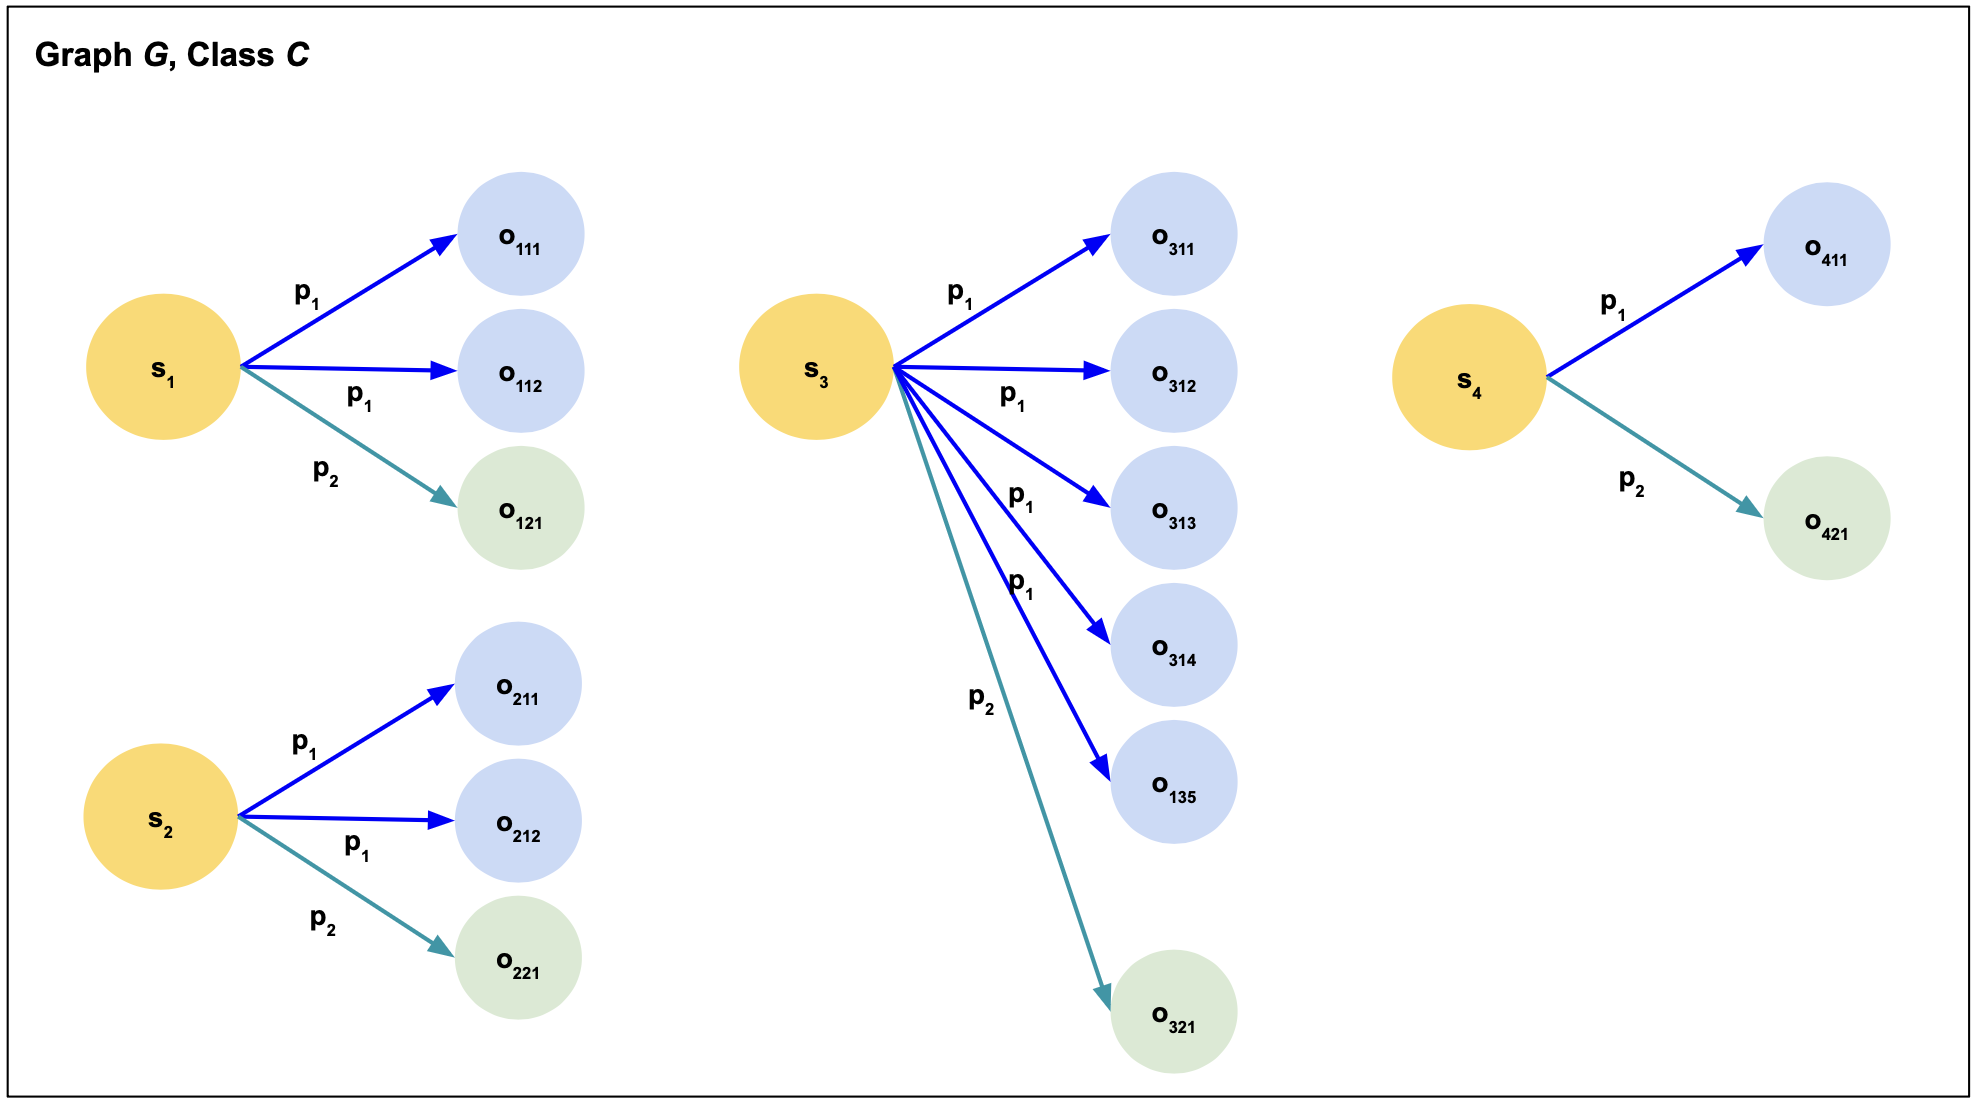
\includegraphics[scale=.3]{Wealth Weighted}
    \caption{Illustration of ...}
    \label{fig:wealth-weighted}
\end{figure}

\paragraph{Wealth based on type of property}
Object properties are other entities besides \(S\) that is connected with \(S\) through a property \(p\). Wealth of \(S\) using bag of properties with only considering the object properties is defined as:
\[
    W_{bag, object}(S, G) = |\{(p,o) | ((S, p, o) \in G) \cap (o \in I)\}|
\]
Data properties are non-object properties that is connected with \(S\) through a property \(p\). Wealth of \(S\) using bag of properties with only considering the data properties is defined as:
\[
    W_{bag, data}(S, G) = |\{(p,o) | ((S, p, o) \in G) \cap (o \in L)\}|
\]

An external ID is a special type of string that is used to represent an entity in an external source. In Wikidata, an ID is element of subclass of \textit{Wikidata property for an identifier} (Q19847637). Just like any other property, an ID is connected with \(S\) through a property \(p\). Let  \(C_{ID,G}\) be a set comprising ID property in graph \(G\). Wealth of \(S\) using bag of properties with only considering the ID properties is defined as:
\[
    W_{bag, ID}(S, G) = |\{(p,o) | ((S, p, o) \in G) \cap (o \in L) \cap (o \in C_{ID,G})\}|
\]

\paragraph{Wealth based on the direction of the link}
In outgoing link type of wealth, the properties that are used in the wealth calculation of an entity \(S\) are those obtained from link with outwards direction from that particular entity \(S\); that is where \(S\) appears to be the subject in the set of triples in graph \(G\). All types of wealth defined before use the notion of outgoing link.

In incoming link type of wealth, the properties that are used in the wealth calculation of an entity \(S\) are those obtained from link with inwards direction to that particular entity \(S\); that is where \(S\) appears to be the object in the set of triples in graph \(G\). To illustrate, let \(N_{bag}(S)\) be a set that comprises all pair of object and predicate/property \((o,P)\) that is connected to \(S\) in incoming direction to \(S\) i.e., \(N_{bag}(S)\) = \(\{(o, p) | (o, p, S) \in G\}\). Then the wealth of \(S\) using bag of properties and the view of incoming link is notated as \(W_{bag, incoming}(S, G)\), and equal to the cardinality of \(N_{bag}(S)\).
\[
    N_{bag, incoming}(S, G) = \{(o,p) | (o, p, S) \in G\}
\]
\[
    W_{bag, incoming}(S, G) = |N_{bag, incoming}(S, G)|
\]

Looking at in \autoref{fig:wealth-type3}, the wealth of entity \(S\) is 1 using outgoing link, which is from the triple \((S, p_1, o1)\). Its wealth is also 1 and using incoming link, which comes from the triple \((o2, p_2, S)\).

Each definition above can be used simultaneously. For example, the wealth of entity \(S\) using set of properties, calculating object and data but not ID properties, and using the direction of outgoing link is denoted by \(W_{set, outgoing, (object \cup data) \cap ID^\complement}(S, G) = |N_{set, outgoing, (object \cup data) \cap ID^\complement}(S, G)|\) with \(N_{set, outgoing, (object \cup data) \cap ID^\complement}(S, G) = \{p | \exists o, (S, p, o) \in G, \cap (o \in ((I \cup L) \cap C_{ID,G}^\complement)\}\)

\subsubsection{Class-Level Wealth}
Let \(C\) be a class that consists of \(m\) distinct entities \(S_1\), \(S_2\), ... \(S_m\) in graph \(G\). The wealth of \(C\) can be be quantified using its constituent entities. It can be described by several measures, such as entity count, mean and median of its entities' wealth, and percentile of its entities's wealth. To illustrate, let a class \(C\) consists of 4 entities  \(S_1\), \(S_2\), \(S_3\), and \(S_4\) from \autoref{fig:wealth-weighted}. We may say class \(C\) has a total wealth of 4 when we look from count of entities.


%% can be formal background and literature studies
\subsection{Insight Model?}

\textit{(Here, should we mention about EDA and simple measures we use in this study? i.e., mean, median mode, etc)}

\paragraph{Exploratory Data Analysis (EDA): Descriptive Statistics Measures.} Descriptive statistics is concerned with the description and summarization of data. It is a summary of a dataset that helps to describe features of data quantitatively (Ross, 2019). To have a general view of wealth distribution of a class, we use the following measures:
\begin{itemize}
  \item measures of central tendency: mean, median, mode
  \item measures of frequency: count, cumulative frequency/percentage
  \item measures of position: quartile, percentile
  \item measures of dispersion: minimum, maximum, range, interquartile range, standard deviation, coefficient of variation, kurtosis
  \item measures of symmetry: skewness
\end{itemize}


\paragraph{Gini Coefficient}

\paragraph{Lorenz Curve} Lorenz curve is a graphical representation of wealth inequality (The Lorenz Curve: What It Tells You About Economic Inequality, 2022). It shows how the wealth is cumulatively distributed, with data points sorted from the poorest to the richest. \textit{(Here, give the example of Lorenz Curve)}. 


\section{Use Cases and Evaluation}

\subsection{Bias in Wikidata}
In this subchapter, analysis is conducted to see whether any particular entity group in Wikidata is underrepresented compared to others. There are 2 analysis done: gender bias and western bias.
\paragraph{Gender Bias in Wikidata}
Gender bias analysis in Wikidata will be performed on 10 Wikidata classes: computer scientist, American singer, American actress/actor, badminton player, businessperson, lawyer, American politician, American writer, American researcher, and American journalist.

To analyze the bias, the first aspect that will be considered is the proportion of each gender in every class. We assume that there are equal numbers of males and females in real-world and this will be the basis to determine if there is any bias in the data. Pearson's chi-square test (goodness-of-fit) is then performed to test the null and alternative hypotheses with significance level of \(\alpha=5\%\) as follows:

\(H_0\): The proportions of males and females in a particular class are equal to the real-world proportion

\(H_1\): The proportions of males and females in a particular class are not equal to the real-world proportion

From \autoref{tab:gender - entity count}, we can see that there are more male entities than female entities in all of the classes. In terms of entity count, the gender gaps in some classes such as American singer, American actress/actor, badminton player, and American writer, are slim. The gender gaps in some other classes are huge, and it can be observed in the classes of computer scientist, businessperson, lawyer, American politician, journalist, and researcher. This phenomenon can also be easily identified through visualization, as exhibited in \autoref{fig:bias histogram-computer scientist}, where the histogram of the female subclass is much smaller compared to the male. Looking at the chi-square test result, as p-value is well below the chosen significance level, the null hypothesis is rejected in all classes. Hence, we consider the difference of entity count to be significant and conclude that the proportions of males and females in each Wikidata class are not the same as the assumed real-world proportion of 50\%-50\%.

However, it is arguable that, for some classes, the gap in entity count between both genders is expected because, in reality, there are more men than women in the workforce, especially in particular fields such as engineering. As a consequence, it is not reasonable if we expect to have an equal number of males and females entities in Wikidata. Therefore, entity count may not be a good measure of bias because of the nature of the data itself. To address this, we need to evaluate other metrics which can quantify the bias on entity-level.

\begin{center}
\small
\begin{threeparttable}
\caption{Entity Count of 10 Wikidata Classes per Gender Category}
\label{tab:gender - entity count}
\begin{tabular}{c c c c c c c c} 

\toprule
    Class Name & Entity & Male & Female & \%Male & \%Female & $\chi$^2 & p-value \\ [0.5ex] 

\midrule
    American actress/actor & 38087 & 21451 & 16636 & 0.56 & 0.44 & 608.72 & 2.13e-134 \\
    American journalist & 17740 & 12223 & 5517 & 0.69 & 0.31 & 2534.97 & 0.0 \\
    American politician & 92901 & 83007 & 9894 & 0.89 & 0.11 & 57539.86 & 0.0 \\
    American researcher & 4867 & 3387 & 1480 & 0.70 & 0.30 & 747.21 & 1.63e-164 \\
    American singer & 15712 & 9027 & 6685 & 0.57 & 0.43 & 349.09 & 6.67e-78 \\
    American writer & 32573 & 19113 & 13460 & 0.59 & 0.41 & 981.07 & 2.34e-215 \\
    Computer scientist & 17914 & 15229 & 2685 & 0.85 & 0.15 & 8783.74 & 0.0 \\
    Badminton player & 25283 & 13377 & 11906 & 0.53 & 0.47 & 85.58 & 2.22e-20 \\
    Businessperson & 74538 & 66706 & 7832 & 0.89 & 0.11 & 46501.76 & 0.0 \\
    Lawyer & 91348 & 80639 & 10709 & 0.88 & 0.12 & 53533.79 & 0.0 \\ [1ex]
\bottomrule

\end{tabular}
\begin{tablenotes}
    \footnotesize
    This table shows the entity count of 10 Wikidata classes per Gender Category. Chi-square test result shows the significance of difference between the entity count of the two genders male and female.
\end{tablenotes}

\end{threeparttable}
\end{center}

The next metrics to be considered are the measures of central tendency and dispersion to see where the wealth distribution is concentrated and how the data spread.

From \autoref{tab:gender - central tendency}, female entities generally have lower values of measure of central tendency (mean, median, mode). These characteristics can also be observed from the histogram in \autoref{fig:bias histogram-computer scientist}: female histograms’ peak and dense area are located on the left of the male’s. The range of property count of females is generally also lower than males. However, there are some classes in which the richest entity is a female. An example for this is the class of American Singer, which is shown by \autoref{fig:bias histogram-american singer}. Though the value of mean, median, and mode of count of properties are lower for female compared to male, the richest entity on that class is a female entity Madonna (Q1744) with bag of property count of 687, with a significant difference with Michael Jackson (Q2831) with bag of property count of 574. We also observed positive values of skewness (skewness > 0) and high kurtosis values (kurtosis > 3) in all classes, denoting the wealth distribution is right skewed and leptokurtic.

\begin{center}
\small
\begin{threeparttable}
\caption{Measures of Central Tendency of 10 Wikidata Classes per Gender Category}
\label{tab:gender - central tendency}
\begin{tabular}{c c c c} 

\toprule
    Class Name & \CellWithForceBreak{Mean \\ (o/m/f)} & \CellWithForceBreak{Median \\ (o/m/f)} & \CellWithForceBreak{Mode \\ (o/m/f)} \\ [0.5ex] 
\midrule
    American actress/actor & 38.96/39.85/37.80 & 29.00/30.00/28.00 & 19/19/22 \\
    American journalist & 30.71/32.44/26.89 & 23.00/25.00/20.00 & 14/14/14 \\
    American politician & 19.22/19.33/18.25 & 15.00/15.00/15.00 & 13/9/13 \\
    American researcher & 23.97/25.00/21.63 & 20.00/21.00/18.00 & 12/12/12 \\
    American singer & 42.78/42.99/42.51 & 31.00/33.00/30.00 & 18/24/15 \\
    American writer & 38.86/42.76/33.33 & 30.00/33.00/26.00 & 19/22/19 \\
    Computer scientist & 24.16/24.50/22.28 & 19.00/19.00/18.00 & 8/8/8 \\
    Badminton player & 21.50/21.25/21.78 & 16.00/16.00/16.00 & 13/13/13 \\
    Businessperson & 16.91/16.83/17.61 & 13.00/13.00/13.00 & 10/10/9 \\
    Lawyer & 22.44/22.98/18.37 & 19.00/19.00/15.00 & 16/16/12 \\
    [1ex]
\bottomrule
\end{tabular}
\begin{tablenotes}
    \footnotesize
    This table shows the measures of central tendency of 10 Wikidata classes per gender category. Each measure will have 3 values: o (overall), m (male), and f (female).
\end{tablenotes}
\end{threeparttable}
\end{center}


\begin{center}
\small
\begin{threeparttable}
\caption{Measures of Dispersion and Symmetry of 10 Wikidata Classes per Gender Category}
\label{tab:gender - dispersion and symmetry}
\begin{tabular}{c c c c c c} 

\toprule
    Class Name & \CellWithForceBreak{Min \\ (o/m/f)} & \CellWithForceBreak{Max \\ (o/m/f)} & \CellWithForceBreak{Std. Deviation \\ (o/m/f)} & \CellWithForceBreak{Skewness \\ (o/m/f)} & \CellWithForceBreak{Kurtosis \\ (o/m/f)} \\ [0.5ex] 
\midrule
    American actress/actor & 4/4/4 & 687/574/687 & 33.89/32.75/35.28 & 4.23/3.54/4.94 & 30.74/21.59/39.53 \\
    American journalist & 4/5/4 & 402/402/353 & 26.84/28.14/23.23 & 4.21/4.18/4.15 & 30.73/30.18/29.38 \\
    American politician & 4/4/4 & 476/476/328 & 14.77/14.77/14.75 & 6.53/6.55/6.40 & 97.36/100.39/72.68 \\
    American researcher & 4/4/4 & 222/222/171 & 16.89/18.19/13.17 & 3.86/3.79/3.45 & 25.67/23.50/26.78 \\
    American singer & 4/4/4 & 687/574/687 & 39.35/35.33/44.21 & 4.09/3.16/4.61 & 29.38/18.24/33.19 \\
    American writer & 4/4/4 & 476/476/425 & 34.12/37.19/28.30 & 3.56/3.29/4.05 & 20.51/17.35/27.82 \\
    Computer scientist & 3/3/3 & 441/441/168 & 19.53/20.18/15.24 & 3.41/3.45/2.20 & 27.66/27.80/9.33 \\
    Badminton player & 4/9/4 & 360/238/360 & 16.09/15.28/16.96 & 4.23/3.89/4.48 & 30.85/22.98/35.97 \\
    Businessperson & 3/3/3 & 574/574/429 & 14.65/14.01/19.27 & 7.73/7.37/8.15 & 130.49/128.49/108.21 \\
    Lawyer & 3/3/3 & 550/550/328 & 16.61/16.91/13.47 & 5.56/5.59/5.23 & 76.02/76.31/64.39 \\[1ex]
\bottomrule
\end{tabular}
\begin{tablenotes}
    \footnotesize
    This table shows the measures of dispersion and symmetry of 10 Wikidata classes per gender category. Each measure will have 3 values: o (overall), m (male), and f (female).
\end{tablenotes}
\end{threeparttable}
\end{center}

\begin{figure}[htp]
\centering 
\subfloat[Histogram and Marginal Distribution Plot of Wealth for Class Computer Scientist\label{fig:bias histogram-computer scientist}]{%
  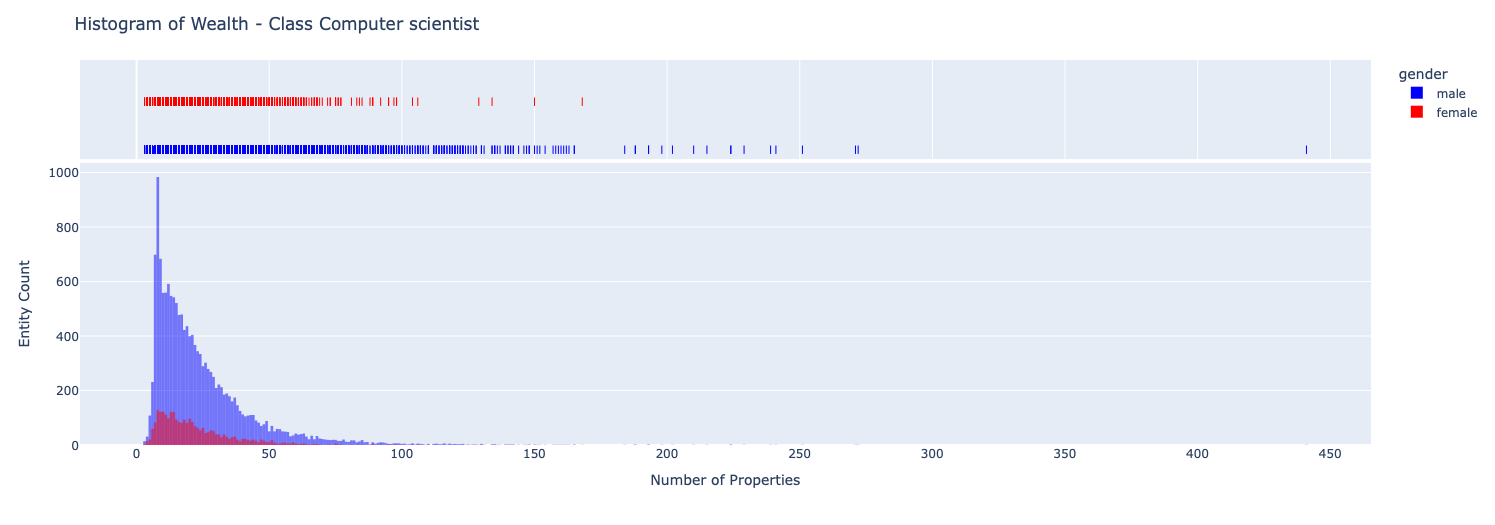
\includegraphics[clip,width=1.0\columnwidth]{Histogram of Wealth - Computer Scientist}%
}

\subfloat[Histogram and Marginal Distribution Plot of Wealth for Class American Singer\label{fig:bias histogram-american singer}]{%
  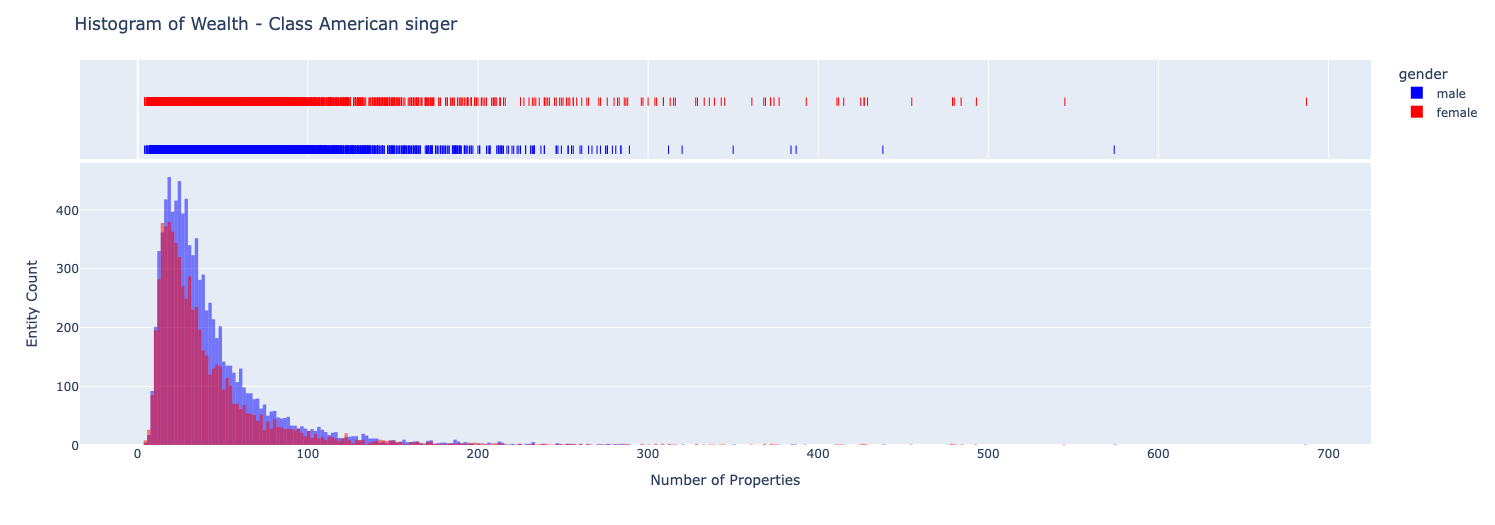
\includegraphics[clip,width=1.0\columnwidth]{Histogram of Wealth - American Singer}%
}

\caption{...}
\label{fig:Histogram of Wealth}

\end{figure}

At a glance we saw female classes are poorer compared to the male classes. To test this, we will use t-test and Welch's test. First, we performed F-test to check if the male and female classes have equal variance. The result of F-test is then used to determine the appropiate test to be used in each class. Those with equal variance will use t-test; otherwise Welch's test is used. Then, we performed the tests to verify the null and alternative hypotheses with significance level of \(\alpha=5\%\) as follows:

\(H_0\): The means of wealth of males and females in a particular class are equal

\(H_1\): The means of wealth of males and females in a particular class are not equal

\begin{center}
\small
\begin{threeparttable}
\caption{F-Test, T-Test, and Welch's Test Result of 10 Wikidata Classes}
\label{tab:gender - mean test}
\begin{tabular}{c c c c c c c} 

\toprule
    Class Name & \CellWithForceBreak{F-Test \\ statistic} & \CellWithForceBreak{F-Test \\ p-value} & \CellWithForceBreak{T-Test \\ statistic} & \CellWithForceBreak{T-Test \\ p-value} & \CellWithForceBreak{Welch's Test \\ statistic} & \CellWithForceBreak{Welch's \\ p-value} \\ [0.5ex] 

\midrule
    American actress/actor & 0.86 & 0.00 & 5.85 & 4.97e-09 & 5.80 & 6.89e-09\\
    American journalist & 1.47 & 1.00 & 12.80 & 2.45e-37 & 13.75 & 1.01e-42 \\
    American politician & 1.00 & 0.55 & 6.86 & 6.90e-12 & 6.87 & 6.94e-12 \\
    American researcher & 1.91 & 1.00 & 6.43 & 1.35e-10 & 7.28 & 4.15e-13 \\
    American singer & 0.64 & 0.00 & 0.75 & 0.45 & 0.73 & 0.47 \\
    American writer & 1.73 & 1.00 & 24.80 & 1.56e-134 & 25.98 & 2.96e-147 \\
    Computer scientist & 1.75 & 1.00 & 5.43 & 5.57e-08 & 6.60 & 4.61e-11 \\
    Badminton player & 0.81 & 0.00 & -2.63 & 8.46e-03 & -2.62 & 8.86e-03 \\
    Businessperson & 0.53 & 0.00 & -4.48 & 7.56e-06 & -3.49 & 4.81e-04 \\
    Lawyer & 1.58 & 1.00 & 27.06 & 1.16e-160 & 32.16 & 8.04e-220 \\
    [1ex]

\bottomrule

\end{tabular}
\begin{tablenotes}
    \footnotesize
    
\end{tablenotes}
\end{threeparttable}
\end{center}

From the test results in \autoref{tab:gender - mean test}, we rejected the null hypothesis in 9 out of 10 class--American singer being the only exception. 7 out of 9 classes are in favor of male. The other 2 classes, American singer and . We concluded that female classes are more likely to have smaller means than male classes.

Here, a new measure is defined: top \(x\)\% male/female relative to the expectation. The value of expectation of a gender in a class is equal to the percentage of that particular in the class. Top \(x\)\% male relative to expectation is the ratio of percentage of male entities in the top \(x\)\% to the expectation. Similarly, top \(x\)\% female relative to expectation is the ratio of percentage of female entities in the top \(x\)\% to the expectation.

When the shape of distribution of male and female of a class is the same (in other word, the wealth is distributed equivalently to male and female entities), then the value of top \(x\)\% relative to expectation should be 1 for both male and female subclasses. A value higher than 1 indicates domination by that particular gender.

\begin{figure}[htp]
\centering 
\subfloat[Ratio of Class Wealth to Expectation per Cumulative Top Percentage - All Classes Average
\label{fig:test1}]{%
  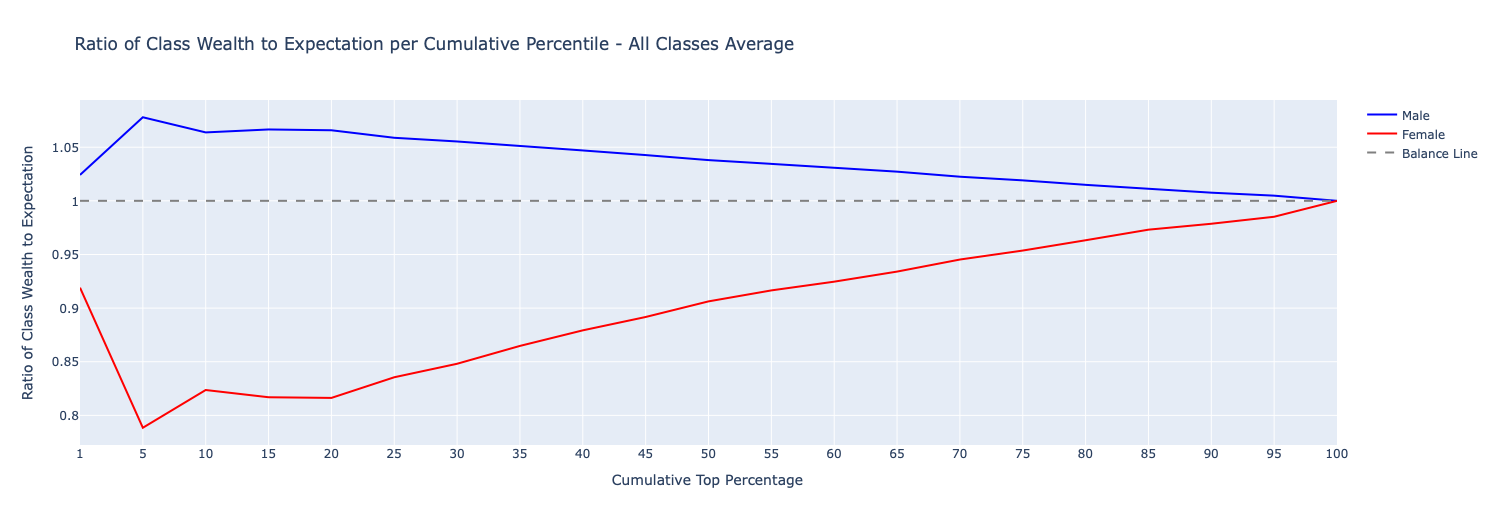
\includegraphics[clip,width=1.0\columnwidth]{Ratio of Class Wealth to Expectation per Cumulative Top Percentage - All Classes Average - Gender}%
}

\subfloat[Ratio of Class Wealth to Expectation per Quantile - All Classes Average\label{fig:test2}]{%
  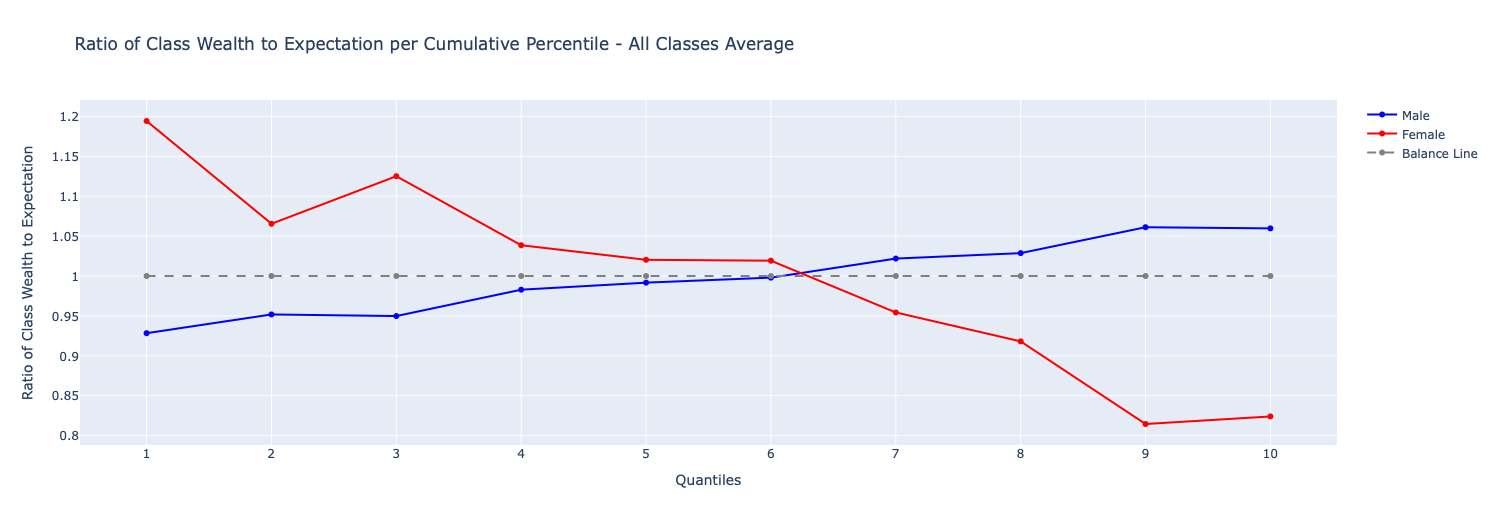
\includegraphics[clip,width=1.0\columnwidth]{Ratio of Class Wealth to Expectation per Quantile - All Classes Average - Gender}%
}

\caption{...}
\label{fig:gender - ratio of gender wealth to expectation}

\end{figure}

From \autoref{fig:gender - ratio of gender wealth to expectation} the value of ratio between top \(x\)\% potion to the expectation in the above tables, we can see that on average, the rich entities are dominated by male. Exceptions are held for 3 classes, that is classes American singer, businessperson, and badminton player. Moreover, as we set bigger portions (higher percentage), the gap of ratio between the two ender in each class decreases i.e. the value of top \(x\)\% relative to expectation of both genders converge to 1.
\paragraph{Western Bias in Wikidata}

Western bias analysis in Wikidata will be performed on 5 Wikidata classes: computer scientist, singer, memorial, university, and river. For each class, we collect the data for the western portion from 8 countries: Canada, France, Germany, Ireland, Poland, Switzerland, the United Kingdom (UK), and the United State of America (USA). For the non-western portion, we also chose 8 countries: China, Egypt, India, Indonesia, Japan, Morocco, Nigeria, and South Africa.

To analyze the bias, the first aspect that will be considered is the proportion of each regional category in every class. We assume that there are equal numbers of western and non-western and this will be the basis to determine if there is any bias in the data. Pearson's chi-square test (goodness-of-fit) is then performed to test the null and alternative hypotheses with significance level of \(\alpha=5\%\) as follows:

\(H_0\): The proportions of western and non-western entities in a particular class are equal

\(H_1\): The proportions of western and non-western entities in a particular class are not equal


\begin{center}
\small
\begin{threeparttable}
\caption{Entity Count of 5 Wikidata Classes per Regional Category}
\label{tab:western - entity count}
\begin{tabular}{c c c c c c c c} 

\toprule
    Class Name & Entity & Western & \CellWithForceBreak{Non- \\ western} & \%Western & \CellWithForceBreak{\%Non- \\ western}& $\chi$^2 & p-value \\ [0.5ex] 
\midrule
    Computer scientist & 6063 & 5446 & 617 & 0.90 & 0.10 & 3846.15 & 0.0 \\
    Singer & 43240 & 31039 & 12201 & 0.72 & 0.28 & 8206.99 & 0.0 \\
    Memorial & 4011 & 3836 & 175 & 0.96 & 0.04 & 3341.54 & 0.0 \\
    University & 6124 & 2398 & 3726 & 0.39 & 0.61 & 287.98 & 1.37e-64 \\
    River & 125567 & 70059 & 55508 & 0.56 & 0.44 & 1686.20 & 0.0 \\
    [1ex]
\bottomrule
\end{tabular}
\begin{tablenotes}
    \footnotesize
    This table shows the entity count of 5 Wikidata classes per regional category. Chi-square test result shows the significance of difference between the entity count of the two genders male and female.
\end{tablenotes}
\end{threeparttable}
\end{center}

In terms of entity count, \autoref{tab:western - entity count} shows that there are big gaps between the westerners and non-westerners in all of the classes. From \autoref{tab:western - central tendency}, non-western entities generally have lower values of measure of central tendency (mean, median, mode). The range of property count of non-westerns is generally also lower than the westerns. Positive values of skewness (skewness > 0) and high kurtosis values (kurtosis > 3) in all classes denote the wealth distribution is right skewed and leptokurtic.

\begin{center}
\small
\begin{threeparttable}
\caption{Measures of Central Tendency of 5 Wikidata Classes per Regional Category}
\label{tab:western - central tendency}
\begin{tabular}{c c c c} 
\toprule
    Class Name & \CellWithForceBreak{Mean \\ (o/w/n)} & \CellWithForceBreak{Median \\ (o/w/n)} & \CellWithForceBreak{Mode \\ (o/w/n)} \\ [0.5ex] 
\midrule
    Computer scientist & 35.00/35.87/27.24 & 29.00/29.00/22.00 & 21/15/16 \\
    Singer & 34.99/39.14/24.43 & 25.00/29.00/18.00 & 15/18/14 \\
    Memorial & 11.04/11.04/11.13 & 9.00/9.00/9.00 & 9/9/9 \\
    University & 23.11/31.61/17.63 & 17.50/24.00/16.00 & 6/6/6 \\
    River & 7.69/8.55/6.60 & 7.00/7.00/6.00 & 7/7/7 \\
    [1ex]
\bottomrule
\end{tabular}
\begin{tablenotes}
    \footnotesize
    This table shows the measures of central tendency of 5 Wikidata classes per regional category. Each measure will have 3 values: o (overall), w (western), and f (non-western).
\end{tablenotes}
\end{threeparttable}
\end{center}

\begin{center}
\small
\begin{threeparttable}
\caption{Measures of Dispersion and Symmetry of 5 Wikidata Classes per Gender Category}
\label{tab:western - dispersion and symmetry}
\begin{tabular}{c c c c c c} 

\toprule
    Class Name & \CellWithForceBreak{Min \\ (o/w/n)} & \CellWithForceBreak{Max \\ (o/w/n)} & \CellWithForceBreak{Std. Deviation \\ (o/w/n)} & \CellWithForceBreak{Skewness \\ (o/w/n)} & \CellWithForceBreak{Kurtosis \\ (o/w/n)} \\ [0.5ex] 
\midrule
    Computer scientist & 4/4/5 & 441/441/145 & 25.15/25.67/18.15 & 3.02/3.02/2.37 & 20.90/20.83/8.49 \\
    Singer & 3/4/3 & 687/687/379 & 33.27/36.60/18.94 & 4.49/4.28/3.15 & 35.56/31.09/21.59 \\
    Memorial & 2/3/2 & 142/142/52 & 5.89/5.82/7.28 & 8.50/8.95/2.98 & 143.57/156.15/12.79 \\
    University & 2/2/2 & 234/234/166 & 20.00/25.88/12.25 & 2.37/1.65/2.22 & 10.34/5.33/12.70 \\
    River & 2/2/2 & 452/452/148 & 5.24/6.46/2.68 & 21.71/19.54/14.67 & 1152.84/868.56/465.42 \\
    [1ex]
\bottomrule
\end{tabular}
\begin{tablenotes}
    \footnotesize
    This table shows the measures of dispersion and symmetry of 5 Wikidata classes per gender category. Each measure will have 3 values: o (overall), w (western), and f (non-western).
\end{tablenotes}
\end{threeparttable}
\end{center}

Out of 5 classes, class of memorial is the only class where the null hypothesis is not rejected. In the other 4 classes, we can see a significant difference between the mean of the two reginal categories, which all are in favor of the western.

\begin{center}
\small
\begin{threeparttable}
\caption{F-Test, T-Test, and Welch's Test Result of 5 Wikidata Classes}
\label{tab:western - mean test}
\begin{tabular}{c c c c c c c} 
\toprule
    Class Name & \CellWithForceBreak{F-Test \\ statistic} & \CellWithForceBreak{F-Test \\ p-value} & \CellWithForceBreak{T-Test \\ statistic} & \CellWithForceBreak{T-Test \\ p-value} & \CellWithForceBreak{Welch's Test \\ statistic} & \CellWithForceBreak{Welch's \\ p-value} \\ [0.5ex] 
\midrule
    Computer scientist & 2.00 & 1.00 & 8.13 & 5.10e-16 & 10.66 & 3.64e-25 \\
    Singer & 3.73 & 1.00 & 42.22 & 0.0 & 54.59 & 0.0 \\
    Memorial & 0.64 & 0.00 & -0.19 & 0.85 & -0.16 & 0.88 \\
    University & 4.46 & 1.00 & 28.40 & 8.23e-167 & 24.73 & 2.12e-123 \\
    River & 5.83 & 1.00 & 66.91 & 0.0 & 72.64 & 0.0 \\
 [1ex]
\bottomrule
\end{tabular}
\begin{tablenotes}
    \footnotesize
\end{tablenotes}
\end{threeparttable}
\end{center}

\begin{figure}[htp]
\centering 
\subfloat[Ratio of Class Wealth to Expectation per Cumulative Top Percentage - All Classes Average
\label{fig:test1 - western}]{%
  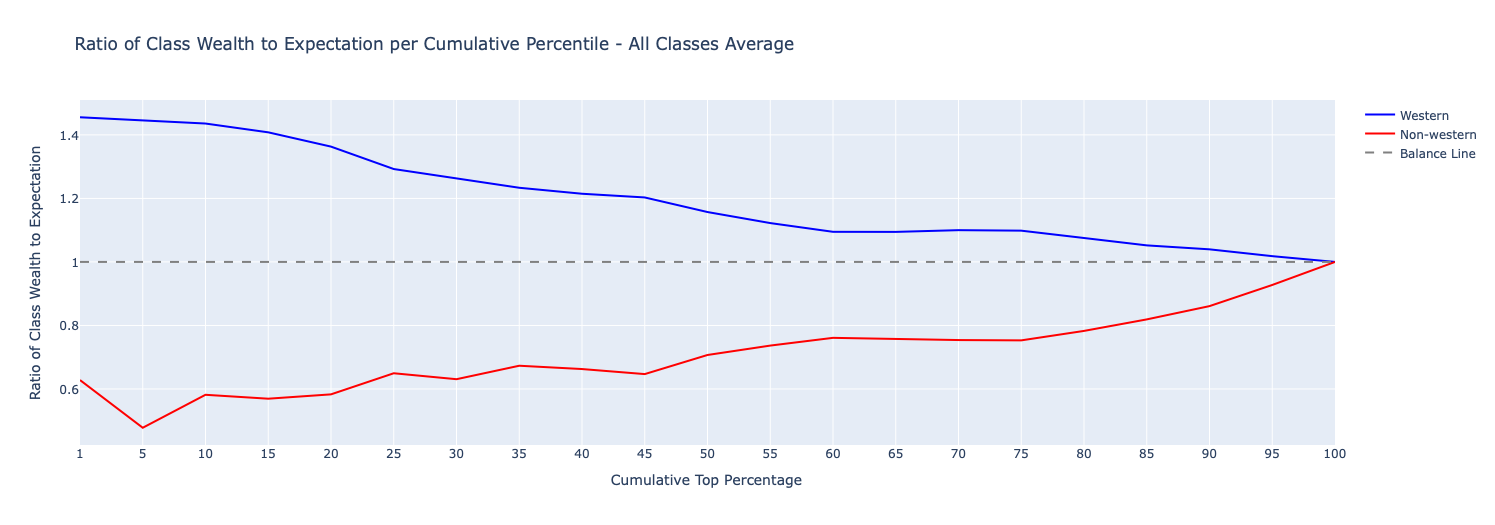
\includegraphics[clip,width=1.0\columnwidth]{Ratio of Class Wealth to Expectation per Cumulative Top Percentage - All Classes Average - Region}%
}

\subfloat[Ratio of Class Wealth to Expectation per Quantile - All Classes Average\label{fig:test2 - western}]{%
  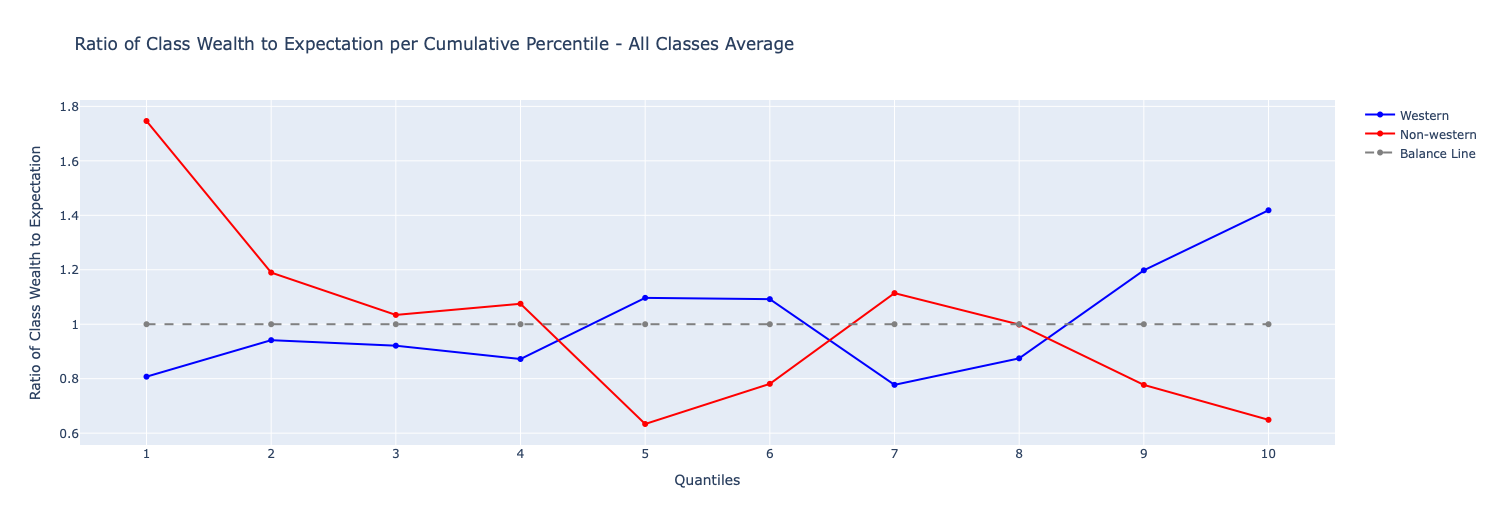
\includegraphics[clip,width=1.0\columnwidth]{Ratio of Class Wealth to Expectation per Quantile - All Classes Average - Gender - Region}%
}

\caption{...}
\label{fig:western - ratio of regional wealth to expectation}

\end{figure}

\subsection{Effect of Type of Wealth on Gini Ratio}
\subsection{Effect of Type of Wealth on Gini Ratio}


\subsection{Proxy of Knowledge Wealth: Real-World Rankings}
- Popularity
- Movie IMDb
- GDP, economic wealth
- Personal net worth

\subsection{(Tentative) Basics of Knowledge Wealth Comparison}

\paragraph{Subclass-to-Subclass Wealth Comparison}
\paragraph{Subclass-to-Superclass Wealth Comparison}
\paragraph{Totally Different Classes Wealth Comparison}

\subsection{(Tentative) Knowledge Wealth Evolution using Wikidata History}

\subsection{(Tentative) Pareto Principle in Wikidata}

\subsection{(Tentative)}
This is additional, if possible. Based on WN notes to use statistical measures for machine learning

\section{Discussion}

TBD

\section{Conclusions}

TBD

\begin{acknowledgments}

TBD

\end{acknowledgments}

\bibliography{mybibliography}

\end{document}